% !TEX root = ../agglo_clust_review.tex

\begin{figure*}[t]
\centering
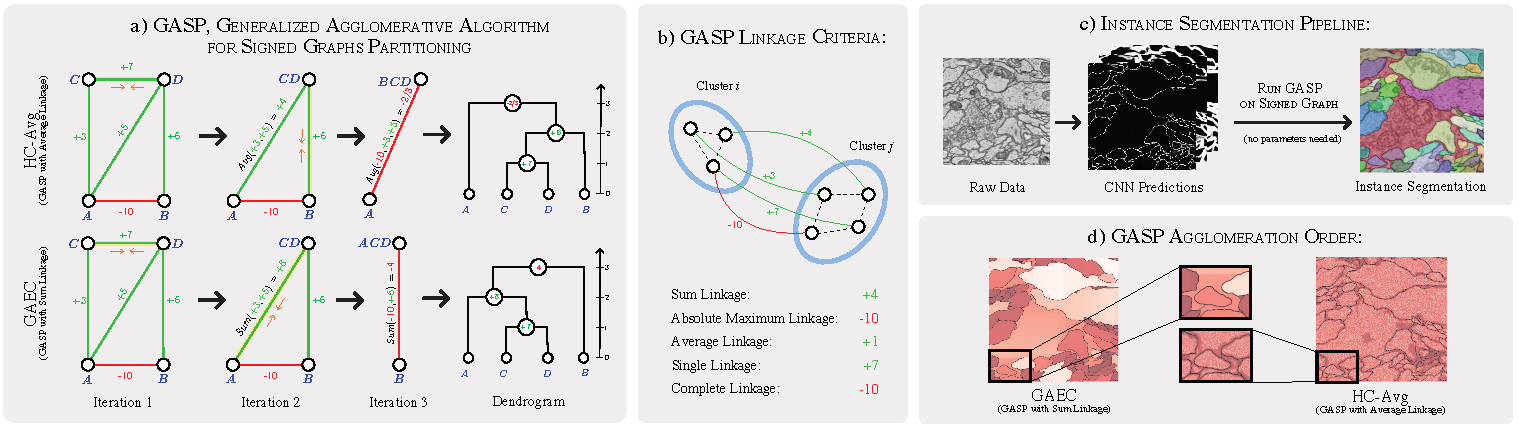
\includegraphics[width=0.98\textwidth]{figs/intro_image_v5.pdf} % left bottom right top
\caption{\textbf{(a)} Some iterations of \algname{}, the proposed Generalized Agglomerative Algorithm for Signed Graph Partitioning, on a toy graph with attractive/positive (green) and repulsive/negative (red) interactions. At each iteration, the yellow edge with highest interaction is contracted (average and sum linkage methods are shown). \textbf{(b)} List of linkage criteria used in this paper (see definitions in Table~\ref{tab:linkage-criteria} below), demonstrated on two small clusters.  \textbf{(c)} Application of \algname{} to instance segmentation: we show raw data from the CREMI 2016 neuron-segmentation challenge and some predictions of our CNN model, where white pixels represent boundary evidence. \textbf{(d)} \algname{} agglomeration order for sum and average linkage: we show which pairs of neighboring pixels were merged first (white), later on (brown/red), or never (black).
\label{fig:intro_figure}}
\end{figure*}

\begin{table*}[t]
    \centering
    \footnotesize
    \begin{subtable}[t!]{\textwidth}\centering
        \begin{tabular}{l |c  c  c  c  c}
        % \multicolumn{1}{c}{}
        % \multirow{2}{*}[-0.5em]{\thead{\textbf{\algname{} linkage criteria} \\ $\,\,\interact(S_u ,S_v)$}}  
        & \thead{Sum\\Linkage} & \thead{Absolute Maximum\\Linkage} & \thead{Average\\Linkage} & \thead{Single\\Linkage} & \thead{Complete\\Linkage} \\
 % \multicolumn{1}{c}{} 
 & $\displaystyle \sum_{e\in E_{ij}} \cost_e$  & $\displaystyle \cost_e$ with $\displaystyle e = \argmax_{t\in E_{ij}} |\cost_t|$ & $\displaystyle \sum_{e\in E_{ij}} \cost_e \bigg/ \big|E_{ij}\big| $ &  $\displaystyle \max_{e\in E_{ij}} \cost_e$ & $\displaystyle \min_{e\in E_{ij}} \cost_e$ \\ \midrule
 % \cmidrule{2-6}

            \thead[r]{GASP on positive-weighted graphs} & \thead{-} &\thead{\textbf{HC-Single}} &\thead{\textbf{HC-Avg}} &\thead{\textbf{HC-Single}} &\thead{\textbf{HC-Complete}} \\
            \thead[r]{GASP on signed graphs} & \thead{GAEC \cite{keuper2015efficient}} & \thead{\textbf{Mutex Watershed} \cite{wolf2018mutex}}& \thead{\textbf{HC-Avg}} &\thead{\textbf{HC-Single}} &\thead{\textbf{HC-Complete}} \\
            \thead[r]{GASP on signed graphs + constraints} & \thead{\colorbox{yellow}{HCC-Sum}} % \thead{Greedy Fixation \cite{levinkov2017comparative}} 
            & \thead{\textbf{Mutex Watershed} \cite{wolf2018mutex}}& \thead{\colorbox{yellow}{HCC-Avg}} &  \thead{\colorbox{yellow}{HCC-Single}} &  \thead{\colorbox{yellow}{HCC-Complete}} \\
            % \multicolumn{2}{c|}{\multirow{2}{*}[-0.5em]{\thead{\textbf{\algname{} linkage criteria} $\,\,\interact(S_u ,S_v)$}}}  & \multirow{2}{*}[-0.5em]{\thead{\textbf{Unsigned Graphs}}} & \multicolumn{2}{c}{\thead{\textbf{Signed Graphs}}}  \\        
            % \multicolumn{2}{c|}{} &  &  \multicolumn{1}{c}{\thead{No Constraints}} & \thead{With Constraints} \\ \midrule
             

            %  Sum: & $\displaystyle \sum_{e\in E_{uv}} \cost_e$ & \thead{Sum Linkage\\Hier. Aggl. Clust.} & \thead{GAEC \cite{keuper2015efficient}} & \thead{Greedy\\Fixation \cite{levinkov2017comparative}} \\ 
            
             


            %  \makecell[r]{Abs. Max:} & 
            % $\displaystyle \cost_e$ with $\displaystyle e = \argmax_{t\in E_{uv}} |\cost_t|$
            %    & \thead{Single Linkage\\Hier. Aggl. Clust.} & \thead{Mutex\\Watershed \cite{wolf2018mutex}} & \thead{Mutex\\Watershed \cite{wolf2018mutex}} \\
             


            %  \makecell[r]{Average:} & $\displaystyle \sum_{e\in E_{uv}} \cost_e \bigg/ \big|E_{uv}\big|  $ & \thead{ Average Linkage\\ Hier. Aggl. Clust.} & \thead{\textbf{NEW}} & \thead{\textbf{NEW}}\\ 

            % Max: & $\displaystyle \max_{e\in E_{uv}} \cost_e$ & \thead{Single Linkage\\Hier. Aggl. Clust.} & \thead{\textbf{NEW}} & \thead{\textbf{NEW}}\\ 

            % Min:& $\displaystyle \min_{e\in E_{uv}} \cost_e$ & \thead{Complete Linkage\\ Hier. Aggl. Clust.}  & \thead{\textbf{NEW}} & \thead{\textbf{NEW}}

        \end{tabular}
    \end{subtable} 
    \caption{Clustering algorithms included in the proposed \algname{} framework, given a linkage criterion, a type of graph (signed or unsigned) and the optional use of cannot-link constraints. New algorithms are highlighted in yellow (hierarchical clustering with constraints, HCC). Algorithms typeset in bold font define an ultrametric on the graph (see Eq.~\ref{eq:UM_def}). Algorithms included in the \TODO{green box}, are weight-shift invariant (see Prop.~\ref{prop:weight_shift_invariant}). 
    We denote as $E_{ij}=(S_i \times S_{j}) \cap E$ the set of edges connecting two clusters $S_i, S_j$. } 
    \label{tab:linkage-criteria}
\end{table*}



\section{Introduction}
In computer vision, the partitioning of weighted graphs has been successfully applied to tasks as diverse as image segmentation, object tracking and pose estimation. 
Most graph clustering methods work with positive edge weights only, which can be interpreted as similarities or distances between the nodes. These methods require users to specify the desired numbers of clusters (as in spectral clustering) or a termination criterion (e.g.\ in iterated normalized cuts) or even to add a seed for each object  (e.g.\ seeded watershed or random walker).  

Other graph clustering methods work with so-called \emph{signed graphs}, which include both positive and negative edge weights corresponding to attraction and repulsion between nodes. The advantage of signed graphs over positive-weighted graphs is that balancing attraction and repulsion allows us to obtain a clustering without defining additional parameters. A canonical formulation of the signed graph partitioning problem is the \emph{multicut} or \emph{correlation clustering} problem \cite{kappes2011globally,chopra1991multiway}. This problem is NP-hard, though many approximate solvers have been proposed \cite{lange2018combinatorial,pape2017solving,beier2016efficient,yarkony2012fast}. The general problem of graph partitioning can also be solved approximately by greedy agglomerative clustering \cite{keuper2015efficient,levinkov2017comparative,wolf2018mutex,kardoostsolving}. 
Agglomerative clustering algorithms for signed graphs have clear advantages: they are parameter-free and efficient. Despite the fact that a variety of these algorithms exist, no overarching study has so far been conducted to compare their robustness and efficiency or to provide guidelines for matching an algorithm to the partitioning problem at hand. 


In this paper, we propose a simple theoretical framework that generalizes over agglomerative algorithms for signed graphs by linking them to hierarchical clustering (HC) on positive-weighted graphs \cite{lance1967general}. This framework defines an underlying basic algorithm and allows us to explore its combinations with different linkage criteria and \emph{cannot-link constraints} (see Fig.~\ref{fig:intro_figure}a-b and Table~\ref{tab:linkage-criteria}). 
We then formally prove that some of the combinations correspond to existing clustering algorithms, and introduce new algorithms for combinations which have not been explored before. By analyzing their theoretical properties, we also show which one of them define ultrametrics on the graph.

We evaluate the algorithms on a large variety of existing and synthetic signed graph clustering problems. 
Moreover, we evaluate all algorithms on \emph{instance segmentation} -- a computer vision task consisting in assigning each pixel of an image to an object instance -- by predicting graph edge weights with a CNN (see Fig.~\ref{fig:intro_figure}).
Our experiments show that the choice of a linkage criterion strongly influences the way how clusters are grown by the agglomerative algorithms, making some linkage methods more suited for certain types of clustering problems.
% We focus our comparison on three of the best-performing algorithms included in our framework, which are based on average, sum, and absolute maximum linkage criteria (see Table~\ref{tab:linkage-criteria}). We highlight their empirical properties by showing how clusters are grown differently depending on the algorithm.
We benchmark the clustering algorithms by focusing on their efficiency, robustness and tendency to over- or under-cluster. 
First, we observe that the tested agglomerative algorithms strongly outperform recently proposed spectral clustering methods. Then,  we also show that average-linkage based agglomerative algorithms achieve state of the art results on the competitive CREMI 2016 challenge for neuron segmentation of 3D electron microscopy image volumes of brain tissue. 

% In Sec.~\ref{sec:spectral_clust}, we also show how \algname{} outperforms spectral clustering methods on the task of neuron segmentation and how on synthetic graphs it achieves similar scores to a recently proposed spectral method for signed graphs. 
% \TODO{Define HC abbrv}

% Our code is available at \url{https://github.com/abailoni/GASP}.






